% 63-16(63쪽) — 도함수 y=f'(x) 의 그래프(x=-3 과 -4 사이에서 x축을 지나 올라가고, 원점에서 x축에 접했다가 다시 올라가 x=3 에서 내려간다). 스캔 화질이 낮아 TikZ 로 다시 그림.
% 라벨과 점선은 원문 그대로 -4 · -3 · -1 · O · 2 · 3 · 4 와 y=f'(x) 만 둔다(f(x) 의 증감은 그림에서 읽는 것이 문항의 조건이므로 그 밖의 값은 적지 않는다).
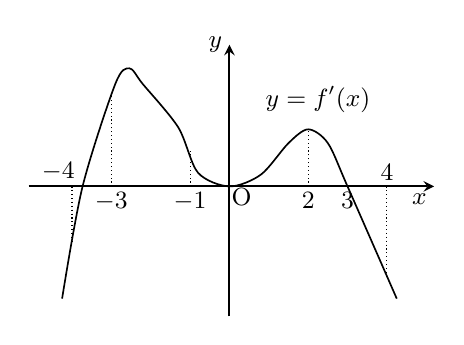
\begin{tikzpicture}[scale=0.5, line width=0.5pt, every node/.style={font=\small}]
  \draw[->, >=stealth, line width=0.7pt] (-5.1,0) -- (5.2,0) node[below left=-1pt] {$x$};
  \draw[->, >=stealth, line width=0.7pt] (0,-3.3) -- (0,3.6) node[left=-1pt] {$y$};
  \node[below right=-1pt, inner sep=1.5pt] at (0,0) {$\mathrm{O}$};
  \draw[densely dotted, line width=0.4pt] (-4,0) -- (-4,-1.45);
  \draw[densely dotted, line width=0.4pt] (-3,0) -- (-3,2.35);
  \draw[densely dotted, line width=0.4pt] (-1,0) -- (-1,0.9);
  \draw[densely dotted, line width=0.4pt] (2,0) -- (2,1.45);
  \draw[densely dotted, line width=0.4pt] (4,0) -- (4,-2.3);
  \draw[line width=0.6pt] plot[smooth] coordinates
    {(-4.25,-2.85) (-3.73,0) (-2.9,2.6) (-2.54,3.0) (-2.2,2.6) (-1.3,1.5) (-0.8,0.35) (0,0) (0.8,0.3) (1.5,1.1) (2.0,1.45) (2.5,1.1) (3.0,0) (4.25,-2.85)};
  \node[above, inner sep=1.5pt] at (2.25,1.75) {$y=f'(x)$};
  \node[above left=-3pt, inner sep=1.5pt] at (-4.02,0.22) {$-4$};
  \node[below, inner sep=2pt] at (-3,0) {$-3$};
  \node[below, inner sep=2pt] at (-1,0) {$-1$};
  \node[below, inner sep=2pt] at (2,0) {$2$};
  \node[below, inner sep=2pt] at (3,0) {$3$};
  \node[above, inner sep=2pt] at (4,0) {$4$};
\end{tikzpicture}
